\documentclass[12pt]{article}
\usepackage[alf]{abntex2cite}
\usepackage[utf8]{inputenc}
\usepackage[portuguese]{babel}
\usepackage{caption}
\usepackage{graphicx}
\usepackage{ragged2e}
\usepackage{indentfirst}
\usepackage{float}
\begin{document}
\begin{table}[h]
    \begin{center}
        
\includegraphics[width=0.09\textwidth]{ufsc_logo.png}
            {\large\textbf{
                \begin{tabular}{l}
                    Universidade Federal de Santa Catarina\\
                    Departamento de Matemática\\
                    Florianópolis - Santa Catarina\\
                \end{tabular}
            }}
            \hrule
        \end{center}
        \small\textbf{Prova 2 de Laboratório de Matemática Computacional - Helena Isola}
\end{table}

\section{Introdução}

Este trabalho tem como ojetivo fazer uma demonstração formal da resolução da parte II da prova 2 da disciplina Laboratório de Matemática Computacional.

Ao longo do trabalho, haverá quatro resoluções de quatro questões distintas, com referências aos exercícios e explicação dos códigos que foram utilizados para resolver as questões.
Na conclusão, será mostrado o desfecho de cada exercício resolvido, com demonstração de exemplos e gráficos. 

\pagebreak
\section{Resolução}

\subsection{Exercício 1}

A questão 1 diz o seguinte:
\emph{"Elabore um aplicativo que determina as raízes de uma equação de segundo grau e que considera todas as possibilidades referentes
ao tipo de raiz. O aplicativo deve mostrar o gráfico da função quadrática correspondente, as coordenadas do vértice, bem como 
informações que o criador do aplicativo julgar relevantes."}

Segue abaixo o código criado para responder ao enunciado e em seguida, a explicação das partes expostas no próprio código:

\begin{figure}[H]
    \begin{center}
        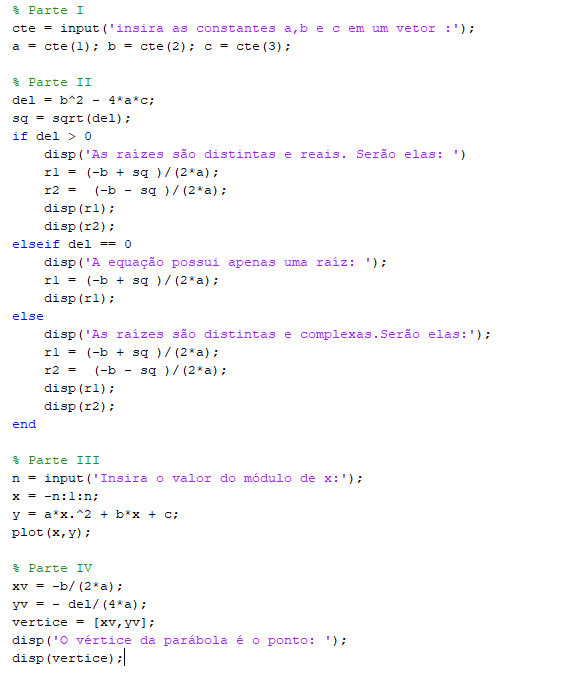
\includegraphics[width=0.8\textwidth]{questao1png.png}
        \label{questao 1}
    \end{center}
\end{figure}

\begin{itemize}
    \item Parte I
   
    Na parte I, há o array chamado \emph{cte} que recebe do usuário um vetor de três variáveis. Tem-se também a o armazenamento em 
    constantes a,b e c os valores de cada posição do vetor \emph{cte}. Estes são o que definimos como coeficientes de uma equação de segundo grau.

    \item Parte II 
    
    Foi definido na parte II uma constante denominada \emph{del}, que representa o discriminante de uma função quadrática, e ele foi calculado utilizando
    os coeficientes definidos pelo usuário na parte I. Em seguida, se tem o cálculo da raiz quadrada de \emph{del}.
    Na estrutura condicional criada, verificamos se o valor de \emph{del} é positivo, nulo ou negativo. Dependendo de cada uma dessas possibilidades, será obtido
    um tipo de resultado diferente.
    \begin{itemize}
        \item Caso \emph{del} seja positivo:
        Quando o discriminante é positivo, se tem consequentemente que a equação quadrática terá duas raízes reais e distintas. Assim, 
        é retornado uma mensagem que afirma qual a natureza das raízes, é feito também o cálculo de cada uma das duas raízes possíveis 
        e depois, elas são retornadas separadamente.

        \item Caso \emph{del} seja nulo:
        Quando o discriminante é nulo, existirá apenas uma raíz como solução da equação de segundo grau. Com mesmo objetivo do item 
        anterior, é retornado umas mensagem que afirma qual a natureza da raíz, é feito também o cálculo dela para depois retornar ela.
        
        \item Caso \emph{del} seja negativo:
        Quando o discriminante é negativo, se tem  que a equação quadrática terá duas raízes complexas e distintas. Assim, 
        é retornado uma mensagem que afirma qual a natureza das raízes, é feito também o cálculo de cada uma das duas raízes possíveis 
        e depois, elas são retornadas separadamente.
    \end{itemize}
\end{itemize}

Concluí-se então o que foi inicialmente pedido no enunciado, já que foi determinado as raízes de uma equação de segundo grau e também,
foi considerado todas as possibilidades referentes ao tipo da raiz.

\begin{itemize}
    \item Parte III
    
    Na parte III, o usuário pode agora inserir qual o range desejado $n$ para os valores de x, tendo em vista que, ao inserir um valor positivo, este será 
    utilizado como um valor de módulo em x, fazendo de x então um vetor que vai de $-n$ até $n$.

    Tendo agora todos os valores de x desejados, é definido y como a equação quadrática e em seguida é plotado o gráfico de y em função de x.

    \item Parte IV
    
    Nesta parte, o objetivo foi encontrar os valores de $x_v$ e $y_v$ correspondentes ao vértice. Depois de calculado, o ponto $P=(x_v, y_v)$ é retornado.
\end{itemize}

\subsection{Exercício 2}

Para a questão 2, tem-se a função 
\begin{equation}
    f(x) = \frac{1}{(x-0.03)^2 + 0.01} + \frac{1}{(x-0.09)^2 + 0.04} - 6
    \label{eq}
\end{equation}

O código para definir um intervalo de x, juntamente com o espaçamento de cada valor de x e a função \ref{eq} é:
\begin{figure}[H]
    \begin{center}
        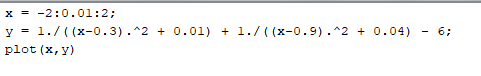
\includegraphics[width=0.8\textwidth]{questao2.png}
    \end{center}
\end{figure}

Agora, desenvolvendo a equação \ref{eq} com o intuito de encontrar uma equação de segundo grau mais explícita
\[ y = \frac{1}{(x-0.03)^2 + 0.01} + \frac{1}{(x-0.09)^2 + 0.04} - 6\] 
\[ y = \frac{1}{x^2 - 0,06x + 0,0009 + 0,01} + \frac{1}{x^2 - 0,18x + 0,0081 + 0.04} - 6\] 
\[ y = \frac{1}{x^2 - 0,06x + 0,0109} + \frac{1}{x^2 - 0,18x + 0,0481} - 6\]



\subsection{Exercício 3}

\subsection{Exercício 4}

\pagebreak
\section{Conclusão}

\subsection{Exercício 1}

Iremos verificar três equações quadráticas diferentes que trazem diferentes resultados que foram apresentados na parte 2.1.

\begin{itemize}
    \item Resultado quando o discriminante é positivo:
    
    \begin{figure}[H]
        \begin{center}
            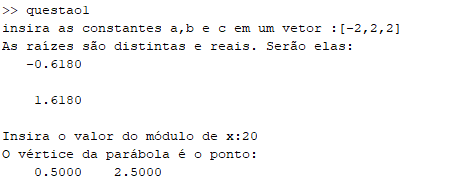
\includegraphics[width=0.8\textwidth]{outputq1-3.png}
        \end{center}
    \end{figure}
    \begin{figure}[H]
        \begin{center}
            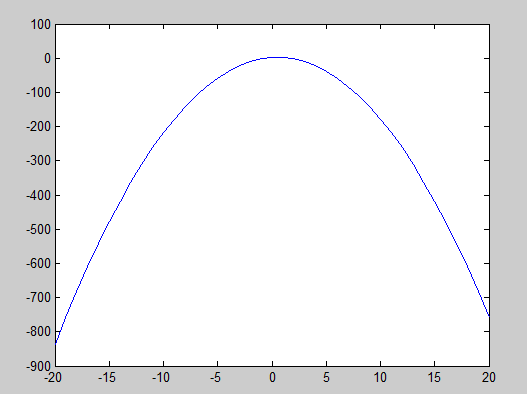
\includegraphics[width=0.6\textwidth]{graficoq1-3.png}
        \end{center}
    \end{figure}

    \item Resultado quando o discriminante é nulo:
    
    \begin{figure}[H]
        \begin{center}
            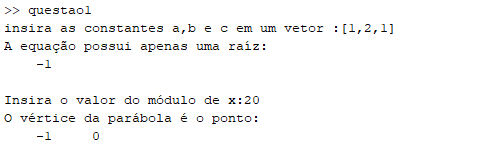
\includegraphics[width=0.8\textwidth]{outputq1-2.png}
        \end{center}
    \end{figure}
    \begin{figure}[H]
        \begin{center}
            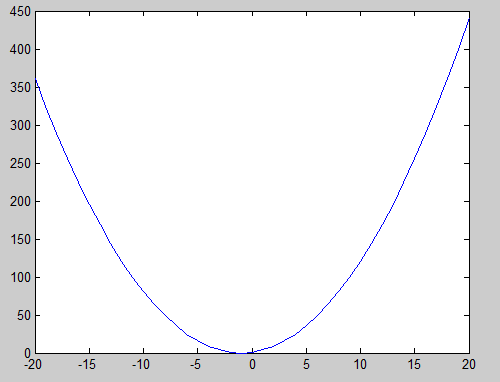
\includegraphics[width=0.6\textwidth]{graficoq1-2.png}
        \end{center}
    \end{figure}

    \item Resultado quando o discriminante é negativo:
    
    \begin{figure}[H]
        \begin{center}
            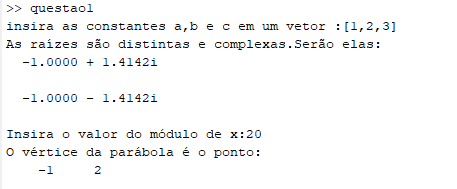
\includegraphics[width=0.8\textwidth]{outputq1-1.png}
        \end{center}
    \end{figure}
    \begin{figure}[H]
        \begin{center}
            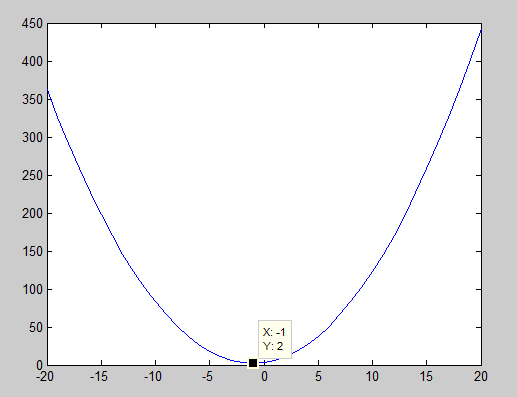
\includegraphics[width=0.6\textwidth]{graficoq1-1.png}
        \end{center}
    \end{figure}
\end{itemize}

\subsection{Exercício 2}

\subsection{Exercício 3}

\subsection{Exercício 4}
\end{document}